\documentclass[12pt,onecolumn]{article}
\usepackage[utf8]{inputenc} % UTF8 input encoding
\usepackage[T2A]{fontenc}   % T2A font encoding for Cyrillic script
\usepackage[russian]{babel} % Russian language support
\usepackage{listings}
\usepackage{float}
\usepackage{mathtools}
\everymath{\displaystyle}
\usepackage{listings} 
\usepackage[usenames]{color}
\usepackage{hyperref}
\usepackage{geometry}
\usepackage{verbatim}
\usepackage{amsmath}
\usepackage{graphicx}
\newcommand{\nparagraph}[1]{\paragraph{#1}\mbox{}\\}
\newcommand{\csection}[1]{
  \addcontentsline{toc}{section}{\textbf{#1}}
  \section*{#1}
  }
\newcommand{\csubsection}[1]{
  \addcontentsline{toc}{subsection}{#1}
  \subsection*{#1}
  }
\newcommand{\csubsubsection}[1]{
  \addcontentsline{toc}{subsubsection}{#1}
  \subsubsection*{#1}
  }
\geometry{
  a4paper,
  top=20mm, 
  right=20mm, 
  bottom=20mm, 
  left=25mm
}
\lstdefinestyle{verilog}{ 
  basicstyle=\small\ttfamily,
  commentstyle=\color{cyan},
  stringstyle=\color{magenta}\ttfamily,
  keywordstyle=\color{blue},
  numbers=left,
  numberstyle=\scriptsize,
  numbersep=5pt,
  frame=single,
  breaklines=true,
  breakatwhitespace=true,
  showstringspaces=false,
  tabsize=4,
  inputencoding=utf8,
  extendedchars=true
}

\begin{document}
\setcounter{tocdepth}{4}
\begin{center}
  Федеральное государственное автономное образовательное учреждение высшего образования "Национальный Исследовательский Университет ИТМО"\\
  Мегафакультет Компьютерных Технологий и Управления\\
  Факультет Программной Инженерии и Компьютерной Техники \\
  
\includegraphics[scale=0.3]{image/itmo.jpg} % нужно закинуть картинку логтипа в папку с отчетом
\end{center}
\vspace{1cm}


\begin{center}
  \large \textbf{Вариант №4}\\
  \textbf{Лабораторная работа 4}\\
  по дисциплине\\
  \textbf{'Функциональная схемотехника'}
\end{center}

\vspace{2cm}

\begin{flushright}
  Выполнил Студент  группы P33102\\
  \textbf{Лапин Алексей Александрович}\\
  Преподаватель: \\
  \textbf{Васильев С.Е.}\\
\end{flushright}

\vspace{9cm}
\begin{center}
  г. Санкт-Петербург\\
  2024г.
\end{center}
\pagestyle{empty}

\newpage
\tableofcontents
\newpage
\csection{Задание}
В лабораторной работе вам предлагается разобраться во внутреннем устройстве простейшего процессорного ядра архитектуры RISC-V. Результатом изучения микроархитектуры процессорного ядра и системы команд RISC-V станут ваши функциональные и нефункциональные модификации ядра.

\textbf{Основное задание:}
\begin{enumerate}
  \item Модифицировать процессорное ядро, в соответствии с вашим вариантом;
  \item Подготовить тестовое окружение системного уровня и убедиться в корректности вашей реализации путём запуска симуляционных тестов.
\end{enumerate}

\textbf{Примечание:} При непосредственном описании ваших модификаций в коде проекта, запрещено использовать симуляционные конструкции и арифметические операции, отличные от сложения и вычитания (то есть, умножение, деление и возведение в степень реализуйте сами посредством описания любого, понравившегося вам, алгоритма). В тестовом окружении использовать симуляционные конструкции и всевозможные арифметические операции можно (и даже нужно).

Варианты с буффером/очередью должны реализовать две команды.
\begin{itemize}
  \item Первая команда - push xN - должна загружать данные из младшей части регистра xN в буффер/очередь.
  \item Вторая команда - pop xN - должна выгружать данные в младшую часть регистра xN.
\end{itemize}

\csection{Микроархитектурная схема модифицированного процессорного ядра}
\begin{figure}[H]
  \centering
  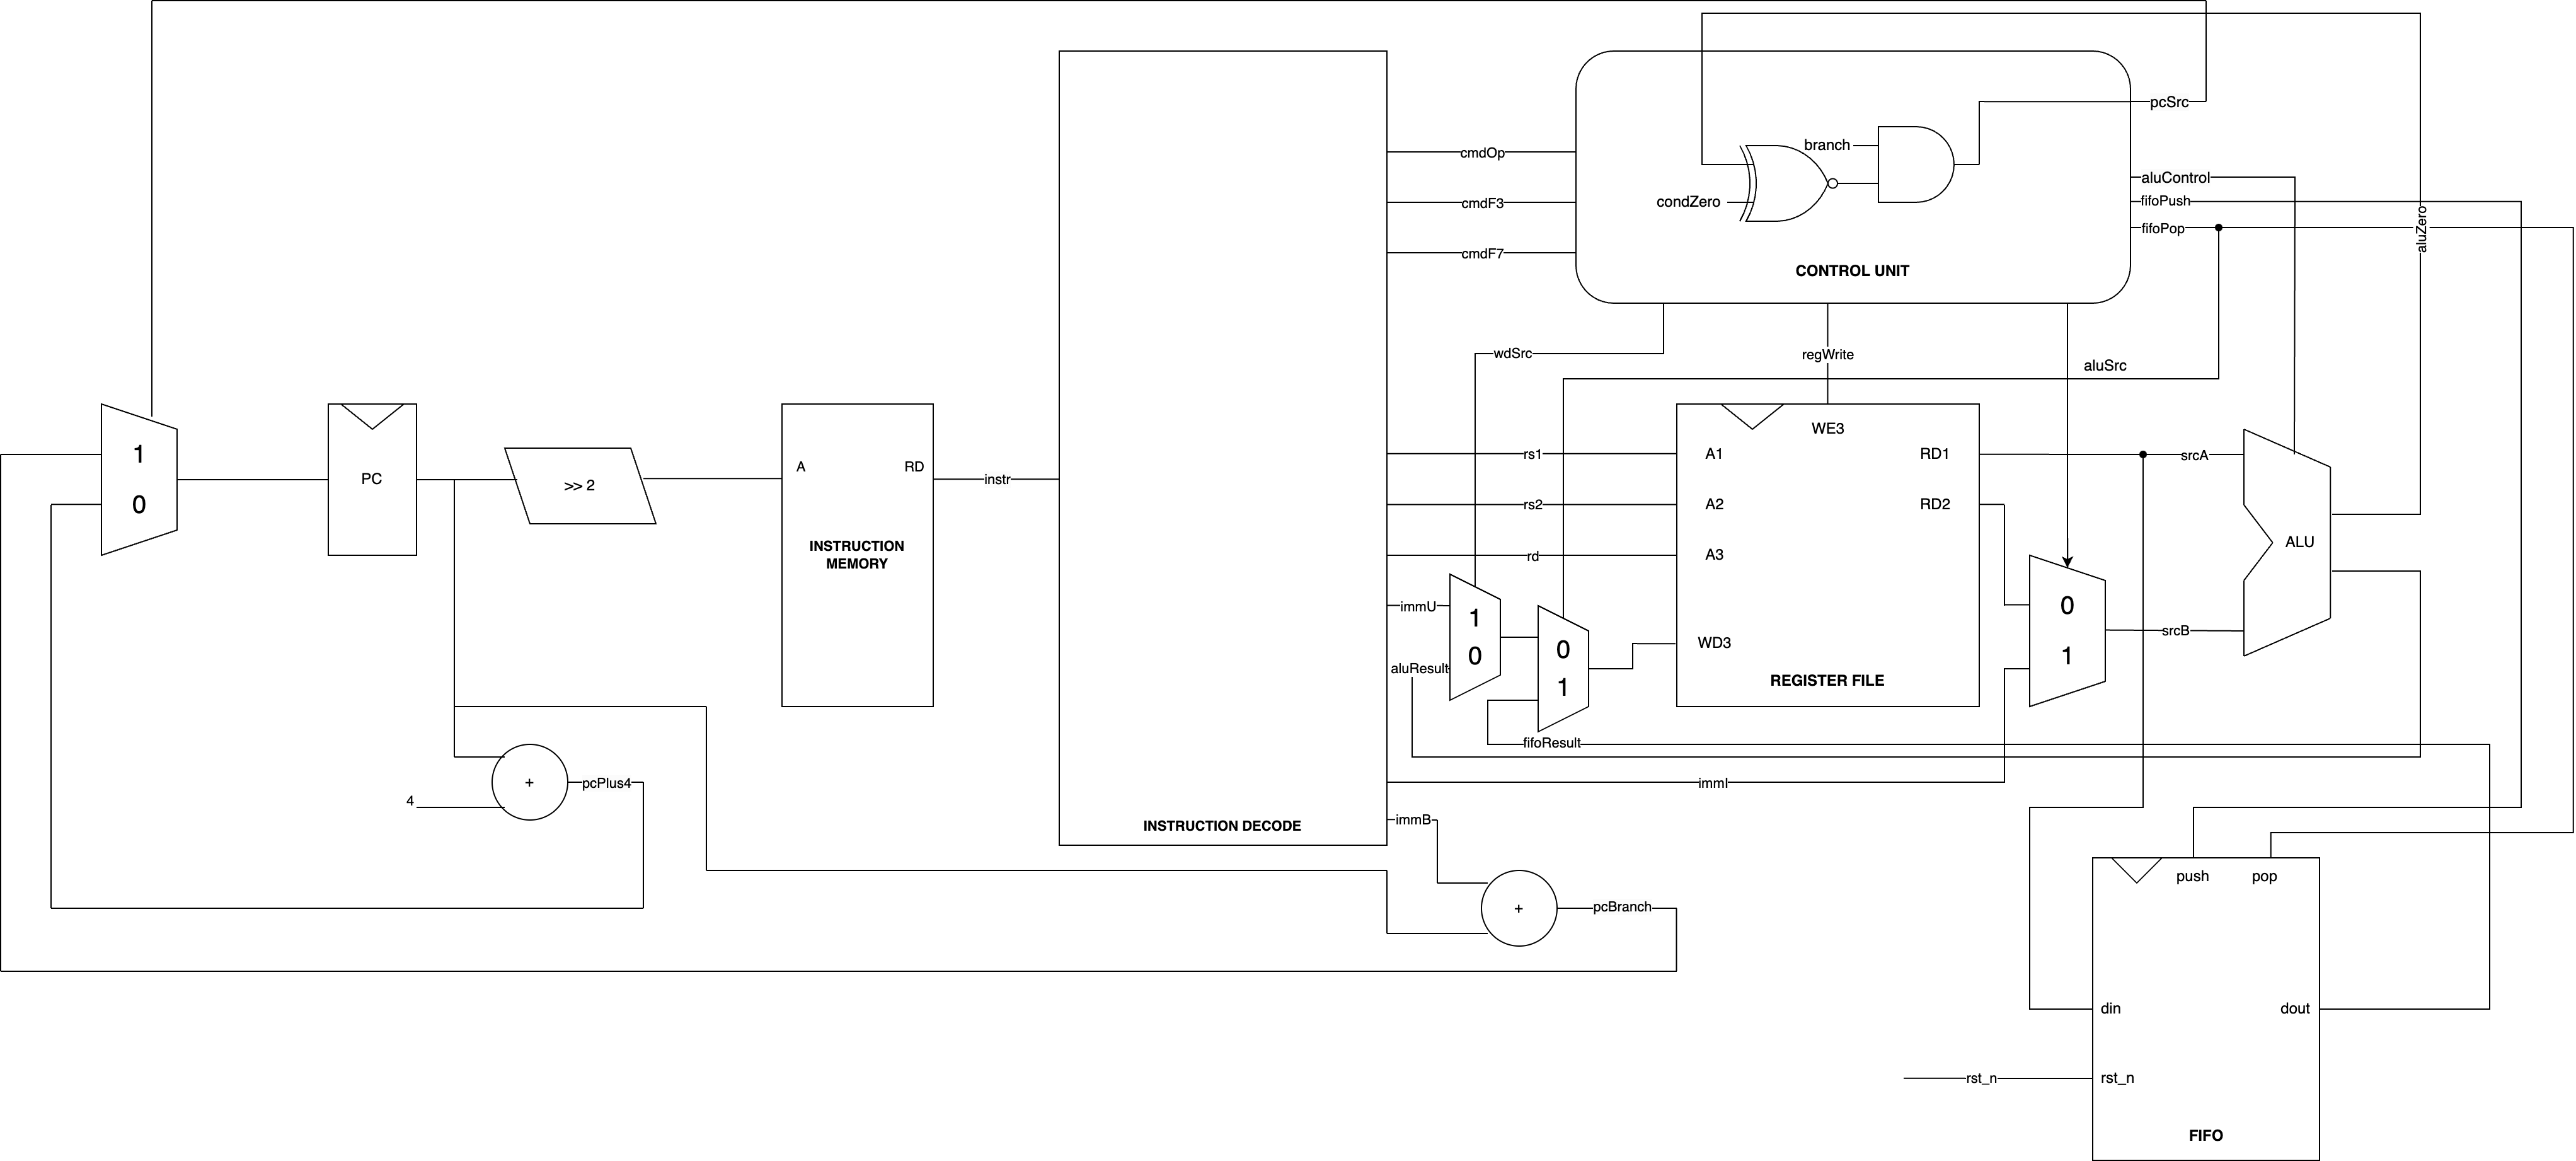
\includegraphics[width=\textwidth]{image/rtl.drawio.png}
  \caption{Микроархитектурная схема процессорного ядра}
\end{figure}

FIFO - добавленный модуль

\csubsection{Описание работы модуля FIFO}

\csubsubsection{1. Входные порты}
\begin{itemize}
  \item \texttt{clk} - тактовый сигнал.
  \item \texttt{rst\_n} - асинхронный сигнал сброса (активный низкий).
  \item \texttt{din} - входные данные шириной \texttt{DATA\_WIDTH} бит.
  \item \texttt{push} - сигнал записи данных в FIFO.
  \item \texttt{pop} - сигнал чтения данных из FIFO.
\end{itemize}

\csubsubsection{2. Описание работы модуля}
Модуль FIFO (First-In-First-Out) реализует очередь с параметризуемой шириной данных (\texttt{DATA\_WIDTH}) и глубиной (\texttt{PTR\_WIDTH}). Основные компоненты модуля включают указатели чтения и записи (\texttt{rd\_ptr} и \texttt{wr\_ptr}), память FIFO (\texttt{mem}) и счетчик элементов (\texttt{count}).

\begin{itemize}
  \item При активном сигнале сброса (\texttt{rst\_n} = 0), указатели чтения и записи, а также счетчик элементов устанавливаются в ноль.
  \item При активном сигнале \texttt{push} и отсутствии переполнения (\texttt{full} = 0), данные из \texttt{din} записываются в память FIFO по адресу \texttt{wr\_ptr}, указатель записи увеличивается на 1, и счетчик элементов увеличивается на 1.
  \item При активном сигнале \texttt{pop} и отсутствии сигнала empty (\texttt{empty} = 0), указатель чтения увеличивается на 1, и счетчик элементов уменьшается на 1.
  \item Выходные данные \texttt{dout} обновляются при активном сигнале \texttt{pop} и отсутствии сигнала empty(\texttt{empty} = 0), принимая значение из памяти FIFO по адресу \texttt{rd\_ptr}.
\end{itemize}

\csubsubsection{3. Выходные порты}
\begin{itemize}
  \item \texttt{dout} - выходные данные шириной \texttt{DATA\_WIDTH} бит.
\end{itemize}

\csubsection{Добавленные управляющие сигналы и их роли}

\csubsubsection{1. fifoPush}
\begin{itemize}
  \item \textbf{Роль}: Этот сигнал управляет операцией записи (push) в FIFO. Если \texttt{fifoPush} установлен, данные из регистра \texttt{rd1} записываются в FIFO.
  \item \textbf{Использование}: В модуле \texttt{sr\_control} сигнал \texttt{fifoPush} активируется при выполнении команды \texttt{RVOP\_PUSH}.
\end{itemize}

\csubsubsection{2. fifoPop}
\begin{itemize}
  \item \textbf{Роль}: {
        \begin{itemize}
          \item Этот сигнал управляет операцией чтения (pop) из FIFO. Если \texttt{fifoPop} установлен, данные из FIFO читаются и передаются на выход.
          \item Этот сигнал определяет источник данных для записи в регистр. Если \texttt{fifoPop} установлен, данные для записи берутся из FIFO, иначе используются данные из ALU или непосредственное значение.
        \end{itemize}
        }
  \item \textbf{Использование}: {
        \begin{itemize}
          \item В модуле \texttt{sr\_control} сигнал \texttt{fifoPop} активируется при выполнении команды \texttt{RVOP\_POP}.
          \item  В модуле \texttt{sr\_cpu} сигнал \texttt{fifoPop} используется для выбора между результатом FIFO (\texttt{fifoResult}) и другими источниками данных (\texttt{immU} или \texttt{aluResult}).
        \end{itemize}
        }
\end{itemize}

\csubsection{Изменения в модулях}

\csubsubsection{Модуль sr\_cpu}
\begin{itemize}
  \item Добавлены новые управляющие сигналы \texttt{fifoPush}, \texttt{fifoPop}.
  \item Добавлен новый модуль \texttt{fifo} для работы с FIFO.
  \item Изменен сигнал \texttt{wd3} для учета нового источника данных \texttt{fifoResult}.
\end{itemize}

\csubsubsection{Модуль sr\_control}
\begin{itemize}
  \item Добавлены новые управляющие сигналы \texttt{fifoPush}, \texttt{fifoPop}.
  \item Добавлены новые команды \texttt{RVOP\_PUSH} и \texttt{RVOP\_POP} для управления FIFO.
\end{itemize}

\csection{Описание добавленных форматов и инструкций}
\begin{figure}[H]
  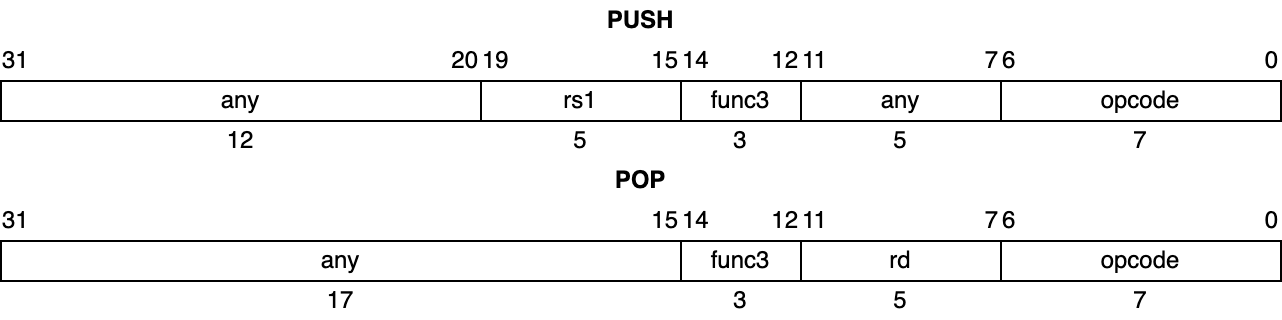
\includegraphics[width=\textwidth]{image/instr.drawio.png}
\end{figure}

\csubsection{Формат инструкции push}

Инструкция `push` используется для сохранения значения регистра в стек.

\begin{itemize}
  \item \textbf{any} (12 бит): Поле, которое может содержать любое значение.
  \item \textbf{rs1} (5 бит): Исходный регистр, значение которого сохраняется в стек.
  \item \textbf{func3} (3 бит): Функциональный код, определяющий тип операции.  В данном случае это `010`. (sw)
  \item \textbf{any} (5 бит): Любые символы, так как результат не сохраняется в регистр.
  \item \textbf{opcode} (7 бит): Код операции. В данном случае это `0100011`, что соответствует инструкции загрузки (load) (мы переиспользуем эту инструкцию).
\end{itemize}

\csubsection{Формат инструкции pop}

Инструкция `pop` используется для извлечения значения из стека и сохранения его в регистр.


\begin{itemize}
  \item \textbf{any} (17 бит): Поле, которое может содержать любое значение.
  \item \textbf{func3} (3 бит): Функциональный код, определяющий тип операции. В данном случае это `010`. (lw)
  \item \textbf{rd} (5 бит): Целевой регистр, в который сохраняется извлеченное значение.
  \item \textbf{opcode} (7 бит): Код операции. В данном случае это `0000011`, что соответствует инструкции загрузки (load) (мы переиспользуем эту инструкцию).
\end{itemize}


\csection{Результаты из отчёта по временным параметрам}
\begin{figure}[H]
  \centering
  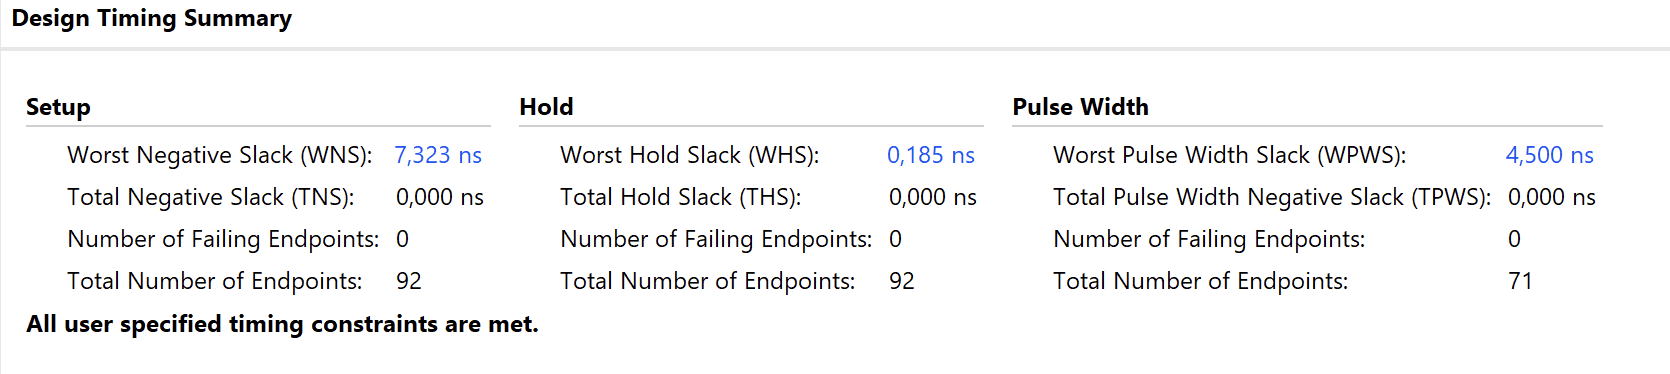
\includegraphics[width=\textwidth]{image/timing.png}
  \caption{Отчет по временным параметрам}
\end{figure}
\begin{itemize}
  \item \textbf{Worst Negative Slack (WNS)}:
        \begin{itemize}
          \item \textbf{Setup}: 7,323 ns
          \item \textbf{Hold}: 0,185 ns
          \item \textbf{Pulse Width}: 4,500 ns
        \end{itemize}
        \textbf{Описание}:
        \begin{itemize}
          \item \textbf{Worst Negative Slack (WNS)} показывает наибольшее отрицательное отклонение времени задержки (slack) для каждого типа временных проверок (setup, hold, pulse width). Отрицательное значение указывает на то, что временные ограничения не выполнены.
          \item \textbf{Setup}: Время задержки между тактовыми сигналами, необходимое для корректной работы схемы.
          \item \textbf{Hold}: Минимальное время, в течение которого сигнал должен оставаться стабильным после тактового сигнала.
          \item \textbf{Pulse Width}: Минимальная ширина импульса тактового сигнала.
        \end{itemize}

  \item \textbf{Total Negative Slack (TNS)}:
        \begin{itemize}
          \item \textbf{Setup}: 0,000 ns
          \item \textbf{Hold}: 0,000 ns
          \item \textbf{Pulse Width}: 0,000 ns
        \end{itemize}
        \textbf{Описание}:
        \begin{itemize}
          \item \textbf{Total Negative Slack (TNS)} показывает суммарное отрицательное отклонение времени задержки для всех конечных точек (endpoints). Значение 0 указывает на то, что все временные ограничения выполнены.
        \end{itemize}

        \csubsubsection{OFFTOP: WNS vs TNS}

        \textbf{Worst Negative Slack (WNS)}
        \begin{itemize}
          \item WNS измеряет самый большой отрицательный запас времени среди всех тайминговых путей в схеме. Это значение показывает, насколько самый плохой путь превышает заданное временное ограничение.
          \item Если WNS равен 2 наносекунды, это означает, что самый критический путь в схеме опаздывает на 2 наносекунды относительно его временного ограничения.
        \end{itemize}

        \textbf{Total Negative Slack (TNS)}
        \begin{itemize}
          \item TNS суммирует отрицательные запасы времени всех тайминговых путей в схеме, которые не соответствуют временным требованиям. Это дает общее представление о том, насколько велика общая задержка по всем путям, которые не укладываются в расписание.
          \item Если TNS равен 10 наносекунд, это означает, что сумма всех отрицательных запасов времени по всем путям составляет 10 наносекунд.
        \end{itemize}

  \item \textbf{Number of Failing Endpoints}:
        \begin{itemize}
          \item \textbf{Setup}: 0
          \item \textbf{Hold}: 0
          \item \textbf{Pulse Width}: 0
        \end{itemize}
        \textbf{Описание}:
        \begin{itemize}
          \item \textbf{Number of Failing Endpoints} показывает количество конечных точек, для которых временные ограничения не выполнены. Значение 0 указывает на то, что все конечные точки соответствуют временным ограничениям.
        \end{itemize}

  \item \textbf{Total Number of Endpoints}:
        \begin{itemize}
          \item \textbf{Setup}: 92
          \item \textbf{Hold}: 92
          \item \textbf{Pulse Width}: 71
        \end{itemize}
        \textbf{Описание}:
        \begin{itemize}
          \item \textbf{Total Number of Endpoints} показывает общее количество конечных точек, для которых проводились временные проверки.
        \end{itemize}
\end{itemize}

\csubsubsection{Выводы из отчета}

\begin{enumerate}
  \item \textbf{Worst Negative Slack (WNS)}:
        \begin{itemize}
          \item Значение WNS для setup времени составляет 7,323 ns, что указывает на значительное отрицательное отклонение. Это может быть проблемой, так как указывает на то, что временные ограничения для setup времени не выполнены.
          \item Значение WNS для hold времени составляет 0,185 ns, что также является отрицательным, но менее критичным.
          \item Значение WNS для pulse width составляет 4,500 ns, что также указывает на нарушение временных ограничений.
        \end{itemize}

  \item \textbf{Total Negative Slack (TNS)}:
        \begin{itemize}
          \item Все значения TNS равны 0, что указывает на то, что в сумме все временные ограничения выполнены.
        \end{itemize}

  \item \textbf{Number of Failing Endpoints}:
        \begin{itemize}
          \item Количество конечных точек, для которых временные ограничения не выполнены, равно 0 для всех типов проверок. Это хороший знак, указывающий на то, что все конечные точки соответствуют временным ограничениям.
        \end{itemize}

  \item \textbf{Total Number of Endpoints}:
        \begin{itemize}
          \item Общее количество конечных точек для setup и hold проверок составляет 92, а для pulse width — 71. Это количество конечных точек, для которых проводились временные проверки.
        \end{itemize}
\end{enumerate}

\csubsubsection{Итог}

Несмотря на то, что Worst Negative Slack (WNS) показывает отрицательные значения для setup, hold и pulse width, общее количество конечных точек, для которых временные ограничения не выполнены, равно 0. Это указывает на то, что все конечные точки соответствуют временным ограничениям, и проект в целом соответствует временным требованиям. Однако, стоит обратить внимание на значительное отрицательное отклонение для setup времени и рассмотреть возможность оптимизации схемы для улучшения временных характеристик.


\csection{Выводы по работе}
\csubsection{Анализ архитектурных решений}
\csubsubsection{2xMux 2-to-1 vs Mux 4-to-1}
При реализации выбора источника данных для записи в регистр можно было пойти двумя путями:
\begin{enumerate}
  \item Сделать четырех входной мультиплексор и расширить сигнал wdSrc до двух бит, что обеспечивает возможность выбора из четырех источников данных.
  \item Сделать два мультиплексора с двумя входами и два сигнала оправления ими. Это обеспечивает возможность выбора из трех источников данных.
\end{enumerate}

В данной работе был выбран второй вариант.

\textbf{Достоинства:}
\begin{itemize}
  \item {\textbf{Избежание лишнего состояния:}

        В 4-разрядном мультиплексоре одно состояние будет лишним, что может привести к неопределенному поведению или необходимости дополнительной логики для обработки этого состояния. Два 2-разрядных мультиплексора позволяют избежать этой проблемы.
        }
  \item {\textbf{Более гибкая конфигурация}
        При необходимости у нас есть отдельные сигналы, которые показывают, "работает" или нет алу и также для fifo.
        }
\end{itemize}
\textbf{Недостатки:}
\begin{itemize}
  \item {\textbf{Усложнение схемы:}

        Требуется два разных сигнала выбора, заместо одного. Это усложняет проектирование схемы.
        }
  \item {\textbf{Потенциальное увеличение стоимости}

        Так как требуется больше мультиплексоров и проводов, это может привести к увеличению стоимости.
        }
  \item {\textbf{Уменьшение скорости работы}

        Использование двух мультиплексоров может увеличить задержку сигнала, так как сигнал должен пройти через два устройства вместо одного.
        }
  \item {\textbf{Потенциальное увеличение потребления энергии}
        Два устройства могут потреблять больше энергии по сравнению с одним
        }
\end{itemize}

При проектировании для меняя важнее было избежать лишнего состояния, поэтому был выбран второй вариант.

\csubsubsection{fifoSign vs fifoPush и fifoPop}
Мы могли бы обединить сигналы fifoPush и fifoPop в один сигнал двух битный fifoSign, который бы определял направление данных в FIFO.
Однако это привило бы к значительному усложнению логики управления.
\csubsubsection{Использование fifoSrc}
Заместо использования fifoPop для двух ролей:
\begin{itemize}
  \item Выбора источника данных для записи в регистр.
  \item Определения направления данных в FIFO.
\end{itemize}
Мы могли бы использовать отдельный сигнал fifoSrc для выбора источника данных для записи в регистр и fifoPop для определения направления данных в FIFO.

\textbf{Достоинства fifoSrc:}
\begin{itemize}
  \item {
        \textbf{Улучшенная читаемость и уменьшение риска ошибок в коде:}

        Разделение сигналов на `fifoSrc` и `fifoPop` делает код более понятным и легким для чтения. Это может упростить процесс отладки. Также разделение функций на разные сигналы уменьшает вероятность ошибок, связанных с неправильной интерпретацией одного сигнала, выполняющего несколько ролей.
        }
  \item {
        \textbf{Улучшенная гибкость:}

        Использование отдельного сигнала `fifoSrc` позволяет более гибко управлять путями записи данных.
        Например если реализовать dout в виде последовательной логики, то мы получим выход только к концу сигнала, когда fifoPop будет уже закрыт.
        Если использовать fifoSrc, то можно считывать данные из fifo в любой момент времени, к примеру на следующем такте после fifoPop.
        }
\end{itemize}

\textbf{Недостатки fifoSrc:}

\begin{itemize}
  \item {
        \textbf{Усложнение схемы:}

        Добавление нового сигнала увеличивает общее количество сигналов в системе, что усложняет схему и потребует больше ресурсов для управления этими сигналами.
        }
  \item {
        \textbf{Увеличение стоимости:}

        Увеличение количества сигналов приводит к увеличению стоимости из-за дополнительных ресурсов.
        }
  \item {
        \textbf{Увеличение потребления энергии:}

        Увеличение количества сигналов может привести к увеличению потребления энергии.
        }
\end{itemize}

Был выбран вариант с использование fifoPop для определения направления данных в FIFO и fifoSrc для выбора источника данных для записи в регистр, так как это упрощает схему и экономит ресурсы.

\csubsubsection{Использовать выход ALU как вход FIFO}
\textbf{Достоинства:}
\begin{itemize}
  \item {
        \textbf{Возможность использовать результат ALU перед записью в FIFO:}

        Использование выхода ALU как входа FIFO позволяет делать вычисления перед записью. Но это потребует изменение формата команды и некоторых архитектурных решений.

        }
  \item {
        \textbf{Потенциальная возможность сокращения управляющих сигнал:}
        Если бы мы использовали fifoSrc и wdScr, то в таком решении можно было бы убрать один из сигналов.
        }
\end{itemize}

\textbf{Недостаки:}
\begin{itemize}
  \item {
        \textbf{Уменьшение скорости работы}

        Использование FIFO в качестве входа ALU может увеличить задержку сигнала, так как сигнал должен пройти через ALU даже если не требуется вычисления.
        }
\end{itemize}

Был выбран вариант использовать FIFO параллельно ALU.

\csubsubsection{Использовать многотактовую реализацию процессора RISC-V}
\textbf{Достоинства:}
\begin{itemize}
  \item {
        \textbf{Потенциально можно увеличить тактовую частоту процессора:}

        За счет разбиения на стадии можно выполнять некоторые операции параллельно, чтобы дать более медленным операциям время. Но так как в данной работе нет модулей, которые работают более одного такта, то это не даст значительных преимуществ.
        }
  \item {
        \textbf{Общая память для данных и комманд:}

        В многотактовой реализации можно использовать одну память для комманд и данных, что может уменьшить количество требуемых ресурсов.
        }
\end{itemize}
\textbf{Недостатоки:}
\begin{itemize}
  \item {
        \textbf{Усложнение схемы:}

        Многотактовая реализация усложняет схему.
        }

  \item {
        \textbf{Большее количество ресурсов:}

        В многотактовой реализации требуется больше регистров, управляющих сигналов и тп.
        }
\end{itemize}
\csubsection{Заключение}
В результате выполнения лабораторной работы были успешно реализованы и протестированы модификации процессорного ядра архитектуры RISC-V. Добавление модуля FIFO и соответствующих команд `push` и `pop` позволило расширить функциональность процессора. Проведенный анализ временных параметров подтвердил соответствие временным требованиям, несмотря на некоторые отрицательные значения WNS. Выбор архитектурных решений был обоснован необходимостью упрощения схемы, избижанием вероятных ошибок при проектировании и улучшением гибкости управления.
\end{document}